\chapter{Strain}





\section{Green-Lagrange Strain}
The Green-Lagrange strain tensor,
\begin{equation}
 \tEbold 
 \defe
 \half (\tCbold - \vid)
 \;\; \Longleftrightarrow \;\;
 \tE_{IJ} 
 \defe 
 \half(\tC_{IJ} - \delta_{IJ}),
\end{equation}
is closely related to the right Cauchy-Green strain tensor
and is often used in defining constitutive
law relationships because the measure, when linearized
about the reference configuration, coincides with the
small strain tensor of linear deformation elasticity, 
denoted~$\ve{\epsilon}$ and defined 
in~(\ref{eq:infinitesimal_strain}).
This relationship can be seen as follows:
\begin{align}
 2 \tEbold 
     &\overset{(\ref{eq:C_in_terms_of_u})}{=} 
     \vid + \Grad \vu + (\Grad \vu)\transpose + 
     (\Grad \vu)\transpose \Grad \vu 
     - \vid,
     \label{eq:E_expanded} \\
 %\ve{\epsilon}  
 2 \tEbold_{\tiny \mbox{LIN}}
     %&\overset{\tiny \mbox{LIN}}{=} 
     &= 
     \Grad \vu + (\Grad \vu)\transpose,
     \label{eq:small_strain}
\end{align}
where the higher-order (quadratic) term in (\ref{eq:E_expanded}) is set
to zero to achieve (\ref{eq:small_strain}).

\section{Euler-Almansi Strain}
The Euler-Almansi strain tensor,
\be
 \tebold 
 \defe 
 \half (\vid - \tbbold^{-1} )
 \;\; \Longleftrightarrow \;\;
 \te_{ij} 
 \defe 
 \half \left(\delta_{ij} - (\tb_{ij})^{-1}\right),
\ee
can likewise be used to approximate the small strain tensor
$\ve{\epsilon}$ by combining (\ref{eq:left_cauchy_green}) and
(\ref{eq:deformation_gradient}) as follows:
\begin{align}
 2 \tebold &=
     \vid - \left[ \Grad \vvarphi 
     (\Grad \vvarphi)\transpose \right]^{-1} \nonumber \\
     &= 
     \delta_{ij} 
       - \left[ \frac{\partial \varphi_i}{\partial X_J}
                \frac{\partial \varphi_j}{\partial X_J}
         \right]^{-1} % \nonumber \\
     =
      \delta_{ij} 
       - \left[ \frac{\partial X_J}{\partial \varphi_i}
                \frac{\partial X_J}{\partial \varphi_j}
         \right] 
	    \nonumber \\ 
     &\overset{(\ref{eq:displacement})}{=}
      \vid 
       - \left[
                (\vid - \grad \vu) (\vid - \grad \vu)\transpose
         \right]
	   \nonumber \\ 
     &=
     \grad \vu + \grad \vu\transpose - 
     \grad \vu \grad \vu\transpose 
     \label{eq:b_expanded} \\
 %\ve{\epsilon}  
 2 \tebold_{\tiny \mbox{LIN}} 
     %&\overset{\tiny \mbox{LIN}}{=} 
     &=
     \grad \vu + (\grad \vu)\transpose,
     \label{eq:small_strain_two}
\end{align}
where higher-order (quadratic) term in (\ref{eq:b_expanded}) is set
to zero to achieve (\ref{eq:small_strain_two}).

\section{Small Strain}
When displacement gradients are small in the reference configuration 
\be
\Grad \vu \ll 1,
\ee 
or in the current configuration, 
\be
\grad \vu \ll 1,
\ee
respectively, the nonlinear gradient terms 
are negligible and the finite strain theory simplifies to small strain
theory, which occurs when finite strain measures are linearized to 
obtain
$\tEbold_{\tiny \mbox{LIN}}$
and 
$\tebold_{\tiny \mbox{LIN}}$
in the previous sections.

Note that we have restricted the gradients of displacement, and not the
displacement $\vu$ itself.  Thus, displacements between the reference and
current configurations can be large (finite), but the gradients of the
displacement either in the reference or current configuration are small.

Section~\ref{section:rb_rotation_strain} will demonstrate that the 
small strain tensors are not suitable to describe motion that
contains finite rotation.  
This makes sense because, in finite rotation, gradients of displacement
are large, not small.  To adequately describe motion that includes 
finite rotation, the fully nonlinear strain measure, 
such as the Seth-Hill strain family 
(see Section~\ref{section:seth_hill}), must be used.

\section{Infinitesimal Strain}
If we further restrict the small strain theory such that the displacement
is small compared to unity, 
\be
\vu \ll 1,
\ee
the infinitesimal strain theory
is obtained, which has no distinction between Lagrangian and Eulerian 
strain tensors.  

In this case, the two small strain tensors, 
$\tEbold_{\tiny \mbox{LIN}}$
and 
$\tebold_{\tiny \mbox{LIN}}$
converge to a single definition of strain, called the infinitesimal
strain tensor $\ve{\epsilon}$, defined as
\be
 \ve{\epsilon} \defe \dst\half(\grad \vu + (\grad \vu)\transpose).
 \label{eq:infinitesimal_strain}
\ee
Note that the $\Grad(\cdot)$ notation has been dropped since the
distinction between the reference and current configurations is 
nonexistent. Also, note that the factor of $\half$ appears because
it then follows that the infinitesimal strain is simply the symmetric
part of the displacement gradient, 
\be
 \ve{\epsilon} = \mbox{\sym}(\grad \vu).
\ee
Finally, note that the finite Lagrangian and Eulerian strain tensors
were defined with the factor of $\half$ so that their expressions, 
once linearized and subject to a small displacement assumption, simplify
to exactly the infinitesimal strain tensor $\ve{\epsilon}$.


\section{Seth-Hill Strain Family}
\label{section:seth_hill}
We return to finite strain definitions, and show that the 
Lagrangian and Eulerian strain tensors described above are two
special cases of a family of finite strain tensors.

Seth and Hill showed that the 
Green-Lagrange and Euler-Almansi 
strain tensors are special cases of the so-called
Seth-Hill family of strain measures, defined as
\be
 \tEbold_{(m)} \defe 
 \left\{ 
	 \begin{tabular}{ll}
	   $\dst\frac{1}{m}\left(\tUbold^m - \vid \right)$ & for $m\neq0$, \\
	   & \\
	   $\ln\tUbold$ & for $m=0$.
	 \end{tabular}
 \right.
 \label{eq:seth_hill}
\ee
The principal stretches $\lambda_I = \ell_k / L_0$, $0 < \lambda_I < \infty$,
allow the strain measure $\tEbold_{(m)}$ to be written as principal
strains, as a function of principal stretch, $f(\lambda_I)$:
\begin{align}
  \tEbold_{(m)} 
  &= \sum_{I=1}^3 f(\lambda_I) \; \veEihat \otimes \veEihat
  \;\;\Longleftrightarrow \;\; 
  \nonumber \\
  & 
  \tE_{(m)\;IJ} = f(\lambda_1)
  \left[ 
  \begin{tabular}{ccc}
  1 & 0 & 0 \\ 
  0 & 0 & 0 \\
  0 & 0 & 0 
  \end{tabular}
  \right] 
  + \; 
  f(\lambda_2)
  \left[ 
  \begin{tabular}{ccc}
  0 & 0 & 0 \\ 
  0 & 1 & 0 \\
  0 & 0 & 0 
  \end{tabular}
  \right] 
  + \; 
  f(\lambda_3)
  \left[ 
  \begin{tabular}{ccc}
  0 & 0 & 0 \\ 
  0 & 0 & 0 \\
  0 & 0 & 1 
  \end{tabular}
  \right],
\end{align}
where the {\bf stretch function}
\be
 f(\lambda_I) \defe
 \left\{ 
	 \begin{tabular}{ll}
	   $\dst\frac{1}{m}\left(\lambda_I^m - 1 \right)$ & for $m\neq0$, \\
	   & \\
	   $\ln(\lambda_I)$ & for $m=0$.
	 \end{tabular}
 \right.
\ee
For integer values of $m \in [-2, 2]$, 
five common strain measures result, listed
in Table~\ref{tab:table_of_strains}, in their three-dimensional and
one-dimensional forms.
\begin{table}[htb]
\caption{Strains obtained from the Seth-Hill family.}
\label{tab:table_of_strains}
\begin{center}
\begin{tabular}{|c|c|c|c|} \hline
 $m$ & {\bf Name} & {\bf 3D} & {\bf 1D} \\ \hline \hline
 & & & \\
 2 & Green-Lagrange 
   & $\tEbold_{(2)} = \dst\frac{1}{2}\left(\tUbold^2 - \vid\right)$ 
   & $\tE_{\tiny\mbox{LAG}} = 
   \dst\frac{1}{2}\left[\left(\dst\frac{\ell}{L_0}\right)^2 - 1\right]$
   \\
   & & & \\ \hline
 & & & \\
 1 & engineering (Biot, nominal)
   & $\tEbold_{(1)} = \tUbold - \vid$
   & $\tE_{\tiny\mbox{ENG}} = \dst\frac{\ell - L_0}{L_0}$
   \\
   & & & \\ \hline
 & & & \\
 0 & log (Hencky, natural)
   & $\tEbold_{(0)} = \ln\tUbold$
   & $\tE_{\tiny\mbox{LOG}} = \ln\left(\dst\frac{\ell}{L_0}\right)$
   \\
   & & & \\ \hline
 & & & \\
 -1 & true 
   & $\tEbold_{(-1)} = \vid - \tUbold^{-1}$
   & $\tE_{\tiny\mbox{TRUE}} = \dst\frac{\ell - L_0}{\ell}$
   \\
   & & & \\ \hline
 & & & \\
 -2 & Euler-Almansi 
   & $\tEbold_{(-2)} = \dst\frac{1}{2}\left(\vid - \tUbold^{-2}\right)$
   & $\tE_{\tiny\mbox{EUL}} = \dst\frac{1}{2}
   \left[ 1 - \left(\dst\frac{L_0}{\ell}\right)^2\right]$
   \\
   & & & \\ \hline
\end{tabular}
\end{center}
\end{table}

As will be seen in Section~\ref{section:conjugates}, 
\begin{itemize}
\item The Green-Lagrange strain tensor 
will be the conjugate of the second Piola-Kirchhoff stress tensor,
\item The deformation gradient will be the conjugate of the first
Piola-Kirchhoff stress tensor,
\item The engineering (Biot, nominal) strain tensor 
will be the conjugate of 
the Jaumann (Biot) stress tensor, 
\item The Euler-Almansi strain tensor will be the conjugate of the 
weighted convected stress tensor.
\end{itemize} 
\clearpage

Figure~\ref{fig:strain_v_stretch}
illustrates the one-dimensional strains as a function of
stretch ratio $\lambda = \ell / L_0$.    
\begin{figure}[htb]
  \begin{center}
    %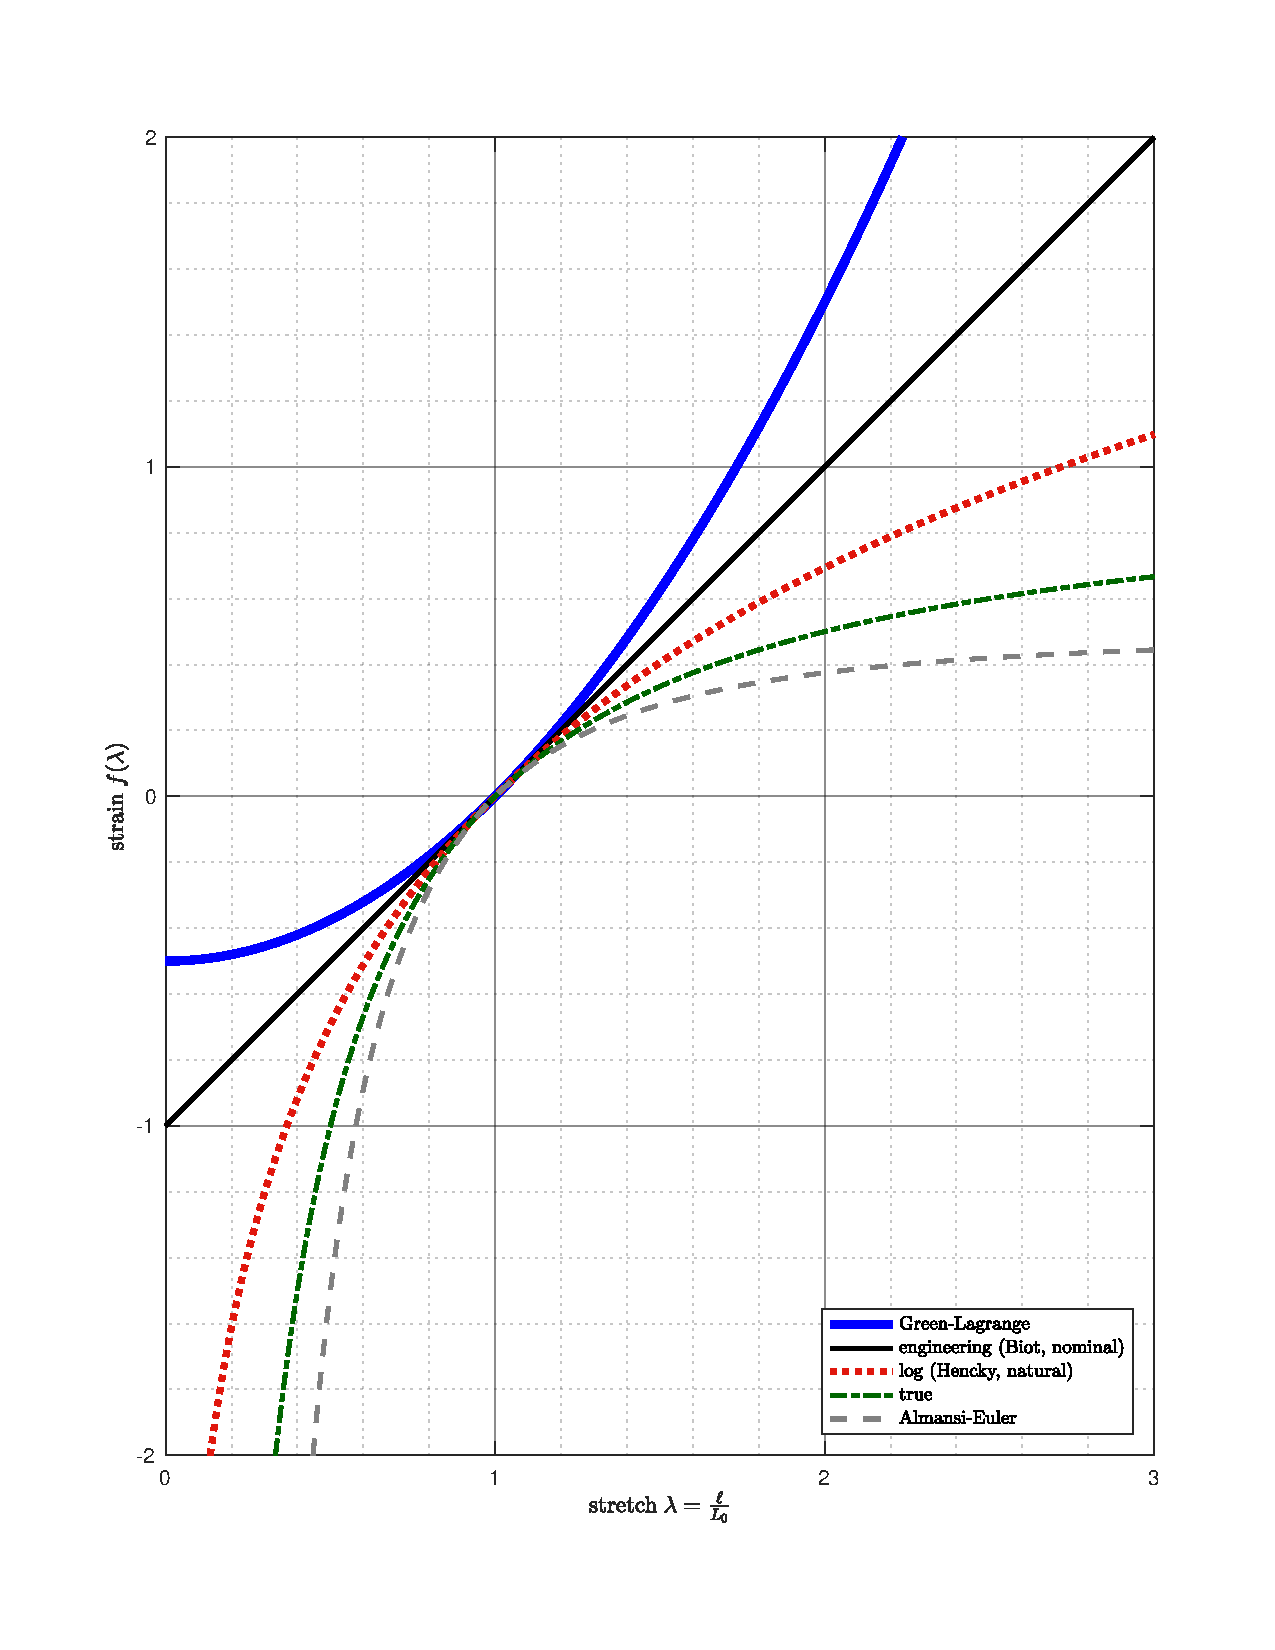
\includegraphics[width=0.8\textwidth,natwidth=612,natheight=792]{fig/strain_v_stretch.pdf}
    %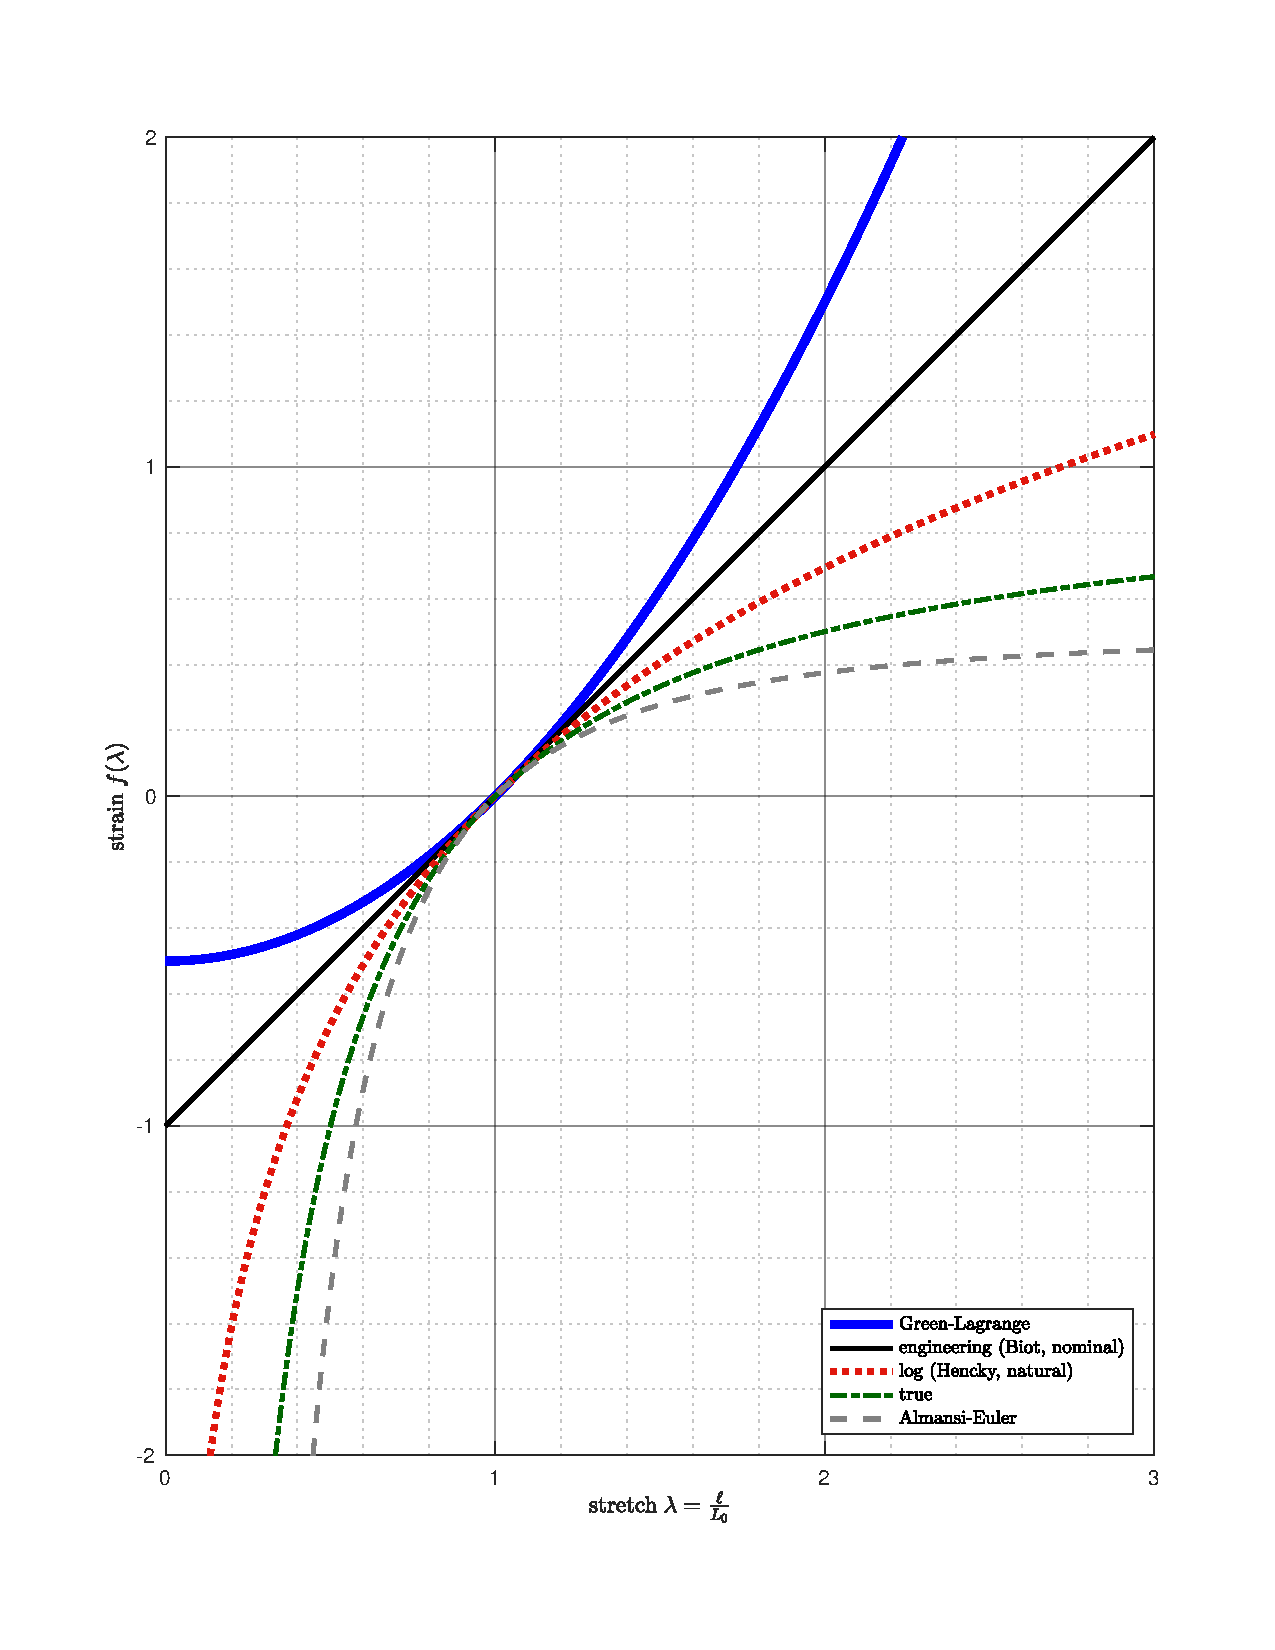
\includegraphics[width=\textwidth,natwidth=612,natheight=792]{fig/strain_v_stretch.pdf}
    %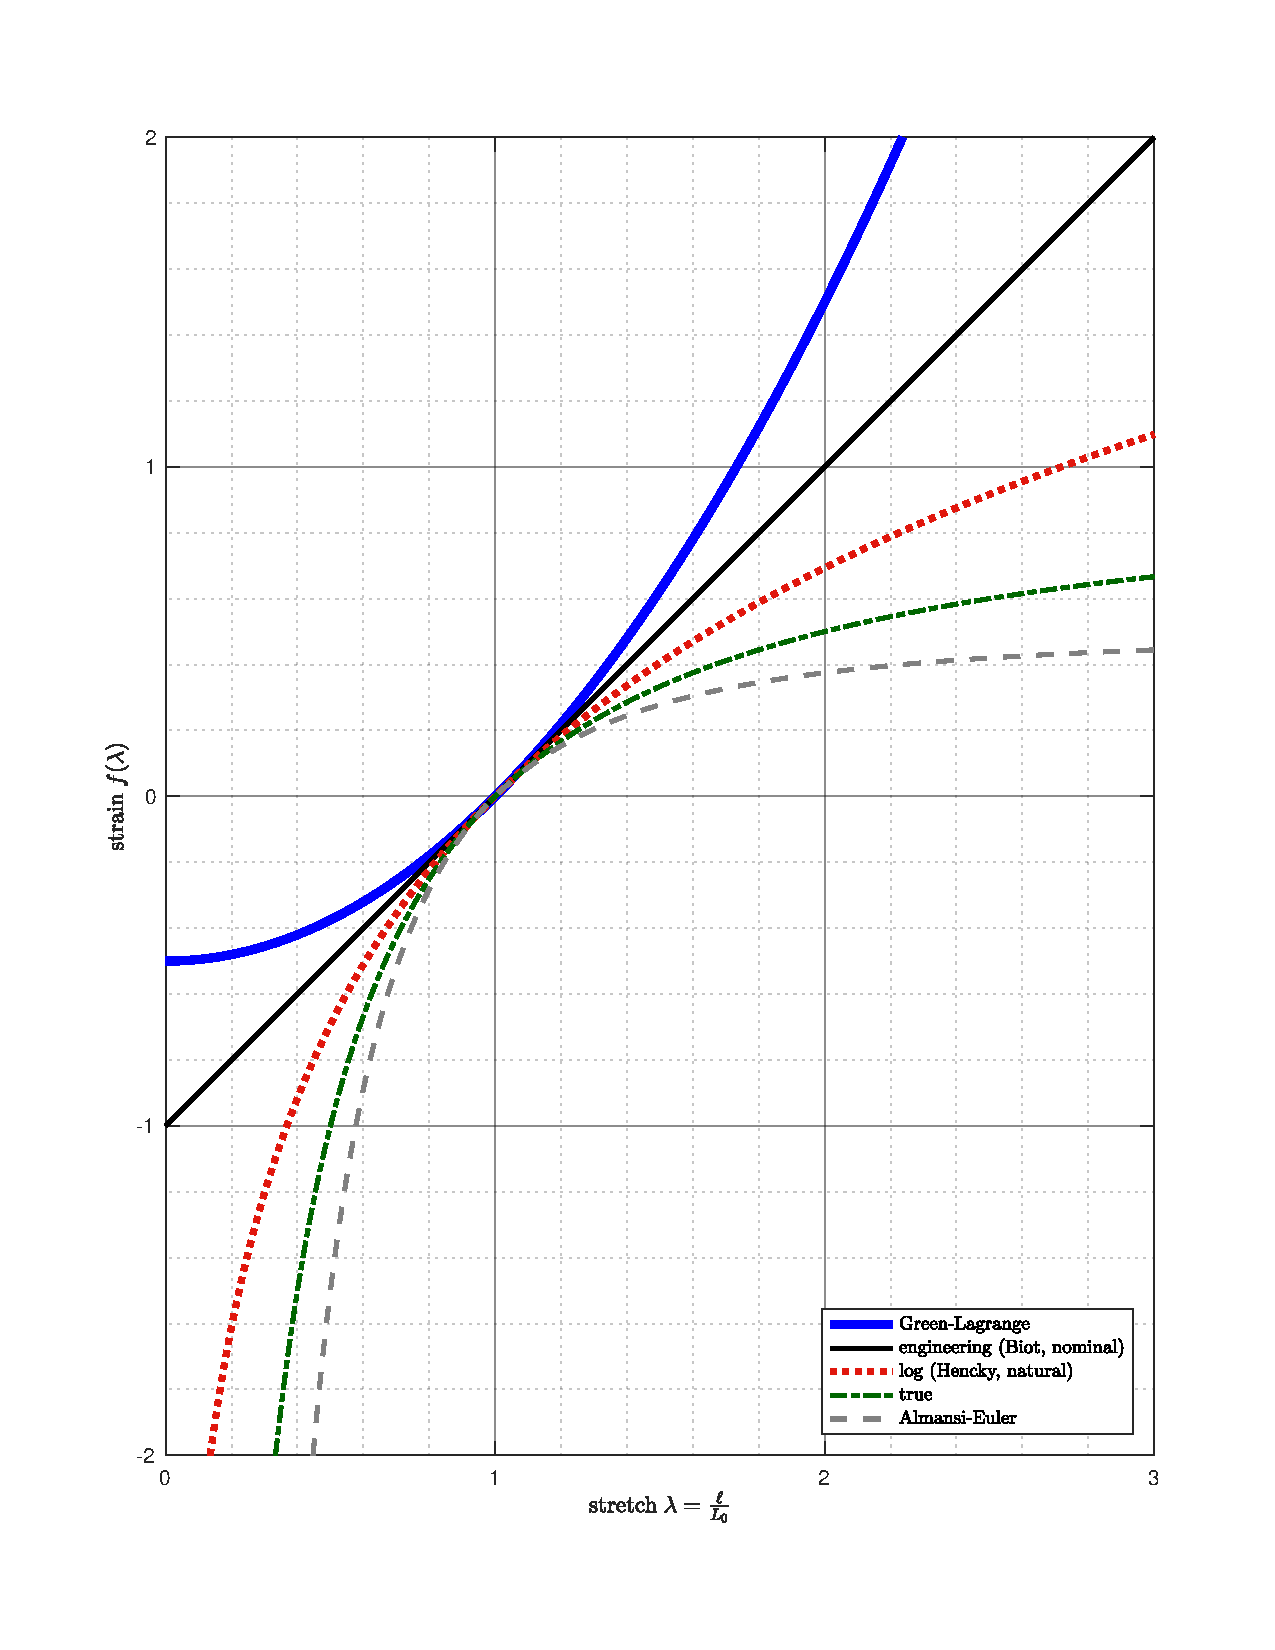
\includegraphics[width=\textwidth]{fig/strain_v_stretch.pdf}
    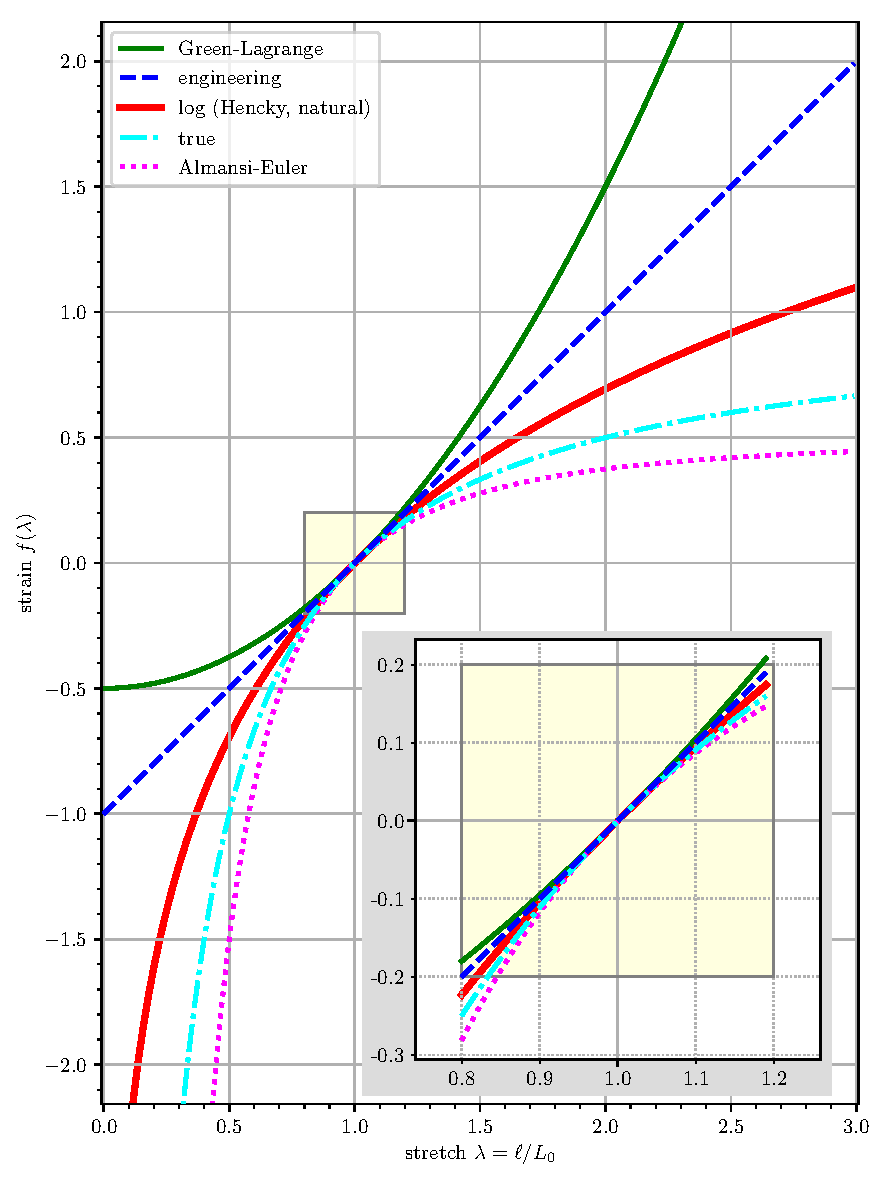
\includegraphics[width=\textwidth]{fig/stretch_strain.pdf}
  \end{center}
  \label{fig:strain_v_stretch}
  \caption{One dimensional strain as a function of stretch ratio.}
\end{figure}
The figure illustrates several results:
\begin{itemize}
 \item For small stretches, $\ell \approx L_0$,
 \begin{itemize}
 \item The stretch ratio is near unity, $\lambda \approx 1$, 
    \item The strain values are small, $f(\lambda) \approx 0$,
    \item The tangent of the strains with respect to the 
    stretch ratio is near unity, $df / d\lambda \approx 1$.
 \end{itemize}
 \item For elongations, $\lambda > 1$, 
 \begin{itemize}
    \item The strain monotonically increases 
    since $df / d\lambda > 0$ when $\lambda > 0$.
 \end{itemize}
 \item For extreme compressions, $\lambda \approx 0$,
 \begin{itemize}
   \item The Green-Lagrange strain goes to a value of $-\half$, 
   \item The engineering (Biot, nominal) strain tensor goes to a value of $-1$, 
   \item The log, true, and Eulerian strains tend to $-\infty$. 
 \end{itemize}
 \item The engineering (Biot, nominal) strain is a linear function of 
 stretch $\lambda$; all other measures are nonlinear functions of
 stretch $\lambda$.
\end{itemize}

\subsection{Reasonable Requirements on the Stretch Function}
This section is based on Neff~(2013),\footnote{Neff, P (2013).  The 
Hencky strain measure the geodesic distance to SO($n$), at 6.}
which presented ``reasonable requirements'' on $f(\lambda) : \realplus
\mapsto \real$.



\begin{tabular}{rl}
$f$ is smooth & true for all in Table~\ref{tab:table_of_strains} \\
$f$ is monotonically increasing & true for all \\
$\left. f \right|_{\lambda = 1} = 0$ & true for all \\
$\left. f' \right|_{\lambda = 1} = 1$ & true for all \\
As $\lambda \rightarrow \infty$, $f \rightarrow +\infty$ & false for true
and
Euler-Almansi strains \\
As $\lambda \rightarrow 0^+$, $f \rightarrow -\infty$ & false for 
Green-Lagrange and engineering strains \\
$-f(\lambda) = f\left(\frac{1}{\lambda}\right)$ & 
true for Hencky and Ba\v{z}ant strains \\
$f(\lambda^{\alpha}) = \alpha f(\lambda)$ & true for only the Hencky strain, 
$\alpha \in \real$
\end{tabular}


Note: the Ba\v{z}ant strain, 
defined as $f(\lambda) = \half\left(\lambda - \frac{1}{\lambda}\right)$, 
is not considered herein.
\clearpage

\section{Strain Tensors and Finite Rotations}
\label{section:rb_rotation_strain}

Because it takes on nonzero values under finite rotation,
the linearized strain tensor 
should not be used for geometrically nonlinear analysis.
These nonzero values are completely artificial and strictly
an artifact of using a linear strain definition with
geometrically nonlinear motions.   This result is shown as follows:

Let $\tRbold = \tRbold(t)$ be a two-dimensional, 
rigid body rotation parameterized by time $t$
and scaled by constant $\omega = 2 \pi$~radians per second.  
Then, the motion $\vvarphi$ of a body can be written as
\be
 \vvarphi(\vX, t) = \tRbold(t) \vX 
 \;\; \Longleftrightarrow \;\;
 \left\{
 \begin{tabular}{c}
 $x_1$ \\
 $x_2$
 \end{tabular}
 \right\}
 = 
 \left[
 \begin{tabular}{rr}
 $\cos \omega t$ & $\sin \omega t$ \\
 $-\sin \omega t$ & $\cos \omega t$ 
 \end{tabular}
 \right]
 \left\{
 \begin{tabular}{c}
 $X_1$ \\
 $X_2$
 \end{tabular}
 \right\}.
\ee
Then the deformation gradient $\tFbold = \tFbold(t)$ is a function of time
alone,
\be
 \tFbold(t)
 \;\; \Longleftrightarrow \;\;
 \tF_{iJ} 
 = 
 \left[
 \begin{tabular}{rr}
 $\tF_{11}$ & $\tF_{12}$ \\
 $\tF_{21}$ & $\tF_{22}$ 
 \end{tabular}
 \right]
 =
 \left[
 \begin{tabular}{rr}
 $\cos \omega t$ & $\sin \omega t$ \\
 $-\sin \omega t$ & $\cos \omega t$ 
 \end{tabular}
 \right].
\ee
The linearized strain tensor is found to be 
\begin{align}
 2 \tEbold_{\tiny \mbox{LIN}}
 &= \Grad \vu + (\Grad \vu)\transpose, \\
 &= \tFbold - \vid + 
     \left(\tFbold - \vid \right)^T, \\
 &= \tF_{iJ} - \delta_{iJ} + \tF_{Ji} - \delta_{Ji}, \\ 
 &= 
 \left[
 \begin{tabular}{rr}
 $\cos \omega t$ & $\sin \omega t$ \\
 $-\sin \omega t$ & $\cos \omega t$ 
 \end{tabular}
 \right]
 +   
 \left[
 \begin{tabular}{rr}
 $\cos \omega t$ & $-\sin \omega t$ \\
 $\sin \omega t$ & $\cos \omega t$ 
 \end{tabular}
 \right]
 -   
 \left[
 \begin{tabular}{rr}
 $2$ & $0$ \\
 $0$ & $2$ 
 \end{tabular}
 \right], \\
 &=
 2 \left( \cos \omega t - 1 \right) \vid.
\end{align}
Now, for small angles, $\omega t \approx 0$, which is
for small deviations $x_1 \approx X_1$, $x_2 \approx X_2$, then
$\tEbold_{\tiny \mbox{LIN}} = \ve{0}$ for rigid body rotations.
However, for arbitrary finite angles, $\omega t \neq 0$,
and the linearized strain tensor
$\tEbold_{\tiny \mbox{LIN}}$ reports nonzero strain for rigid
body rotations, which is nonsensical.

A correct strain tensor will report zero strain for rigid body
rotations.  One such strain tensor is the fully nonlinear 
Green-Lagrange
strain tensor.  This result is shown as follows:
\begin{align}
 2 \tEbold &= \tFbold\transpose\tFbold - \vid \\
 &= 
 \left[
 \begin{tabular}{rr}
 $\cos \omega t$ & $-\sin \omega t$ \\
 $\sin \omega t$ & $\cos \omega t$ 
 \end{tabular}
 \right]
 \left[
 \begin{tabular}{rr}
 $\cos \omega t$ & $\sin \omega t$ \\
 $-\sin \omega t$ & $\cos \omega t$ 
 \end{tabular}
 \right]
 -   
 \left[
 \begin{tabular}{rr}
 $1$ & $0$ \\
 $0$ & $1$ 
 \end{tabular}
 \right] = \ve{0}. 
\end{align}


